% **************************************************
% Document Class Definition
% **************************************************
\documentclass[%
    paper=A4,               % paper size --> A4 is default in Germany
    twoside=true,           % onesite or twoside printing
    openright,              % doublepage cleaning ends up right side
    parskip=half,           % spacing value / method for paragraphs
    chapterprefix=true,     % prefix for chapter marks
    11pt,                   % font size
    headings=normal,        % size of headings
    bibliography=totoc,     % include bib in toc
    listof=totoc,           % include listof entries in toc
    titlepage=on,           % own page for each title page
    captions=tableabove,    % display table captions above the float env
    chapterprefix=false,    % do not display a prefix for chapters
    appendixprefix=false,    % but display a prefix for appendix chapter
    draft=false,            % value for draft version
]{scrreprt}%


% **************************************************
% Setup YOUR thesis document in this file !
% **************************************************
% !TEX root = my-thesis.tex


% **************************************************
% Files' Character Encoding
% **************************************************
\PassOptionsToPackage{utf8}{inputenc}
\usepackage{inputenc}


% **************************************************
% Information and Commands for Reuse
% **************************************************
\newcommand{\thesisTitle}{Lernen und Studieren (LuSt) - Teil 1}
\newcommand{\thesisName}{Marcel Fraas}
\newcommand{\thesisSubject}{Fragen zur Hausarbeit}
\newcommand{\thesisDate}{24. Februar 2020}
\newcommand{\thesisVersion}{Draft}

\newcommand{\thesisFirstReviewer}{Eva Zeller}
\newcommand{\thesisFirstReviewerUniversity}{\protect{Friedrich-Alexander-Universität Erlangen-Nürnberg (FAU)}}
\newcommand{\thesisFirstReviewerDepartment}{Institut für Lern-Innovation}

% \newcommand{\thesisSecondReviewer}{John Doe}
% \newcommand{\thesisSecondReviewerUniversity}{\protect{Clean Thesis Style University}}
% \newcommand{\thesisSecondReviewerDepartment}{Department of Clean Thesis Style}

% \newcommand{\thesisFirstSupervisor}{Jane Doe}
% \newcommand{\thesisSecondSupervisor}{John Smith}

\newcommand{\thesisUniversity}{\protect{Universität Bayreuth}}
\newcommand{\thesisUniversityDepartment}{}
\newcommand{\thesisUniversityInstitute}{}
\newcommand{\thesisUniversityGroup}{Virtuelle Hochschule Bayern}
\newcommand{\thesisUniversityCity}{Bayreuth}
\newcommand{\thesisUniversityStreetAddress}{Universitätsstr. 30}
\newcommand{\thesisUniversityPostalCode}{95447}


% **************************************************
% Debug LaTeX Information
% **************************************************
%\listfiles


% **************************************************
% Load and Configure Packages
% **************************************************
\usepackage[english]{babel} % babel system, adjust the language of the content
\PassOptionsToPackage{% setup clean thesis style
    figuresep=colon,%
    hangfigurecaption=false,%
    hangsection=true,%
    hangsubsection=true,%
    sansserif=false,%
    configurelistings=true,%
    colorize=full,%
    colortheme=unigreen,%
    configurebiblatex=true,%
    bibsys=biber,%
    bibfile=bib-refs,%
    bibstyle=alphabetic,%
    bibsorting=nty,%
}{cleanthesis}
\usepackage{cleanthesis}

\hypersetup{% setup the hyperref-package options
    pdftitle={\thesisTitle},    %   - title (PDF meta)
    pdfsubject={\thesisSubject},%   - subject (PDF meta)
    pdfauthor={\thesisName},    %   - author (PDF meta)
    plainpages=false,           %   -
    colorlinks=false,           %   - colorize links?
    pdfborder={0 0 0},          %   -
    breaklinks=true,            %   - allow line break inside links
    bookmarksnumbered=true,     %
    bookmarksopen=true          %
}



% **************************************************
% Document CONTENT
% **************************************************
\begin{document}

% uncomment the following command to fill up pages with
% whitespace instead of aligning the first and last lines
% of a page (see \raggedbottom vs. \flushbottom)
%\raggedbottom

% --------------------------
% rename document parts
% --------------------------
%\renewcaptionname{ngerman}{\figurename}{Abb.}
%\renewcaptionname{ngerman}{\tablename}{Tab.}
\renewcaptionname{english}{\figurename}{Fig.}
\renewcaptionname{english}{\tablename}{Tab.}


% --------------------------
% Front matter
% --------------------------
\pagenumbering{roman}			% roman page numbing (invisible for empty page style)
\pagestyle{empty}				% no header or footers
% !TEX root = ../my-thesis.tex
%
% ------------------------------------  --> cover title page
\begin{titlepage}
	\pdfbookmark[0]{Cover}{Cover}
	\flushright
	\hfill
	\vfill
	{\LARGE\thesisTitle \par}
	\rule[5pt]{\textwidth}{.4pt} \par
	{\Large\thesisName}
	\vfill
	\textit{\large\thesisDate} \\
	Version: \thesisVersion
\end{titlepage}


% ------------------------------------  --> main title page
\begin{titlepage}
	\pdfbookmark[0]{Titlepage}{Titlepage}
	\tgherosfont
	\centering

	% {\Large \thesisUniversity} \\[4mm]
	
\includegraphics[width=6cm]{gfx/ubt-logo} \\[10mm]
	
\includegraphics[width=6cm]{gfx/vhb-logo} \\[2mm]
	% \textsf{\thesisUniversityDepartment} \\
	% \textsf{\thesisUniversityInstitute} \\
	% \textsf{\thesisUniversityGroup} \\

	\vfill
	{\large \thesisSubject} \\[5mm]
	{\LARGE \color{ctcolortitle}\textbf{\thesisTitle} \\[10mm]}
	{\Large \thesisName} \\

	\vfill
	\begin{minipage}[t]{.27\textwidth}
		\raggedleft
		\textit{Reviewer}
	\end{minipage}
	\hspace*{15pt}
	\begin{minipage}[t]{.65\textwidth}
		{\Large \thesisFirstReviewer} \\
	  	{\small \thesisFirstReviewerDepartment} \\[-1mm]
		{\small \thesisFirstReviewerUniversity}
	\end{minipage} \\[5mm]
	% \begin{minipage}[t]{.27\textwidth}
	% 	\raggedleft
	% 	\textit{2. Reviewer}
	% \end{minipage}
	\hspace*{15pt}
	% \begin{minipage}[t]{.65\textwidth}
	% 	{\Large \thesisSecondReviewer} \\
	%   	{\small \thesisSecondReviewerDepartment} \\[-1mm]
	% 	{\small \thesisSecondReviewerUniversity}
	% \end{minipage} \\[10mm]
	% \begin{minipage}[t]{.27\textwidth}
	% 	\raggedleft
	% 	\textit{Supervisors}
	% \end{minipage}
	% \hspace*{15pt}
	% \begin{minipage}[t]{.65\textwidth}
	% 	\thesisFirstSupervisor\ and \thesisSecondSupervisor
	% \end{minipage} \\[10mm]

	\thesisDate \\

\end{titlepage}


% ------------------------------------  --> lower title back for single page layout
\hfill
\vfill
{
	\small
	\textbf{\thesisName} \\
	\textit{\thesisUniversityGroup} \\
	\textit{\thesisTitle} \\
	\thesisSubject, \thesisDate \\
	% Reviewers: \thesisFirstReviewer\ and \thesisSecondReviewer \\
	% Supervisors: \thesisFirstSupervisor\ and \thesisSecondSupervisor \\[1.5em]
	\textbf{\thesisUniversity} \\
	\thesisUniversityStreetAddress \\
	\thesisUniversityPostalCode\ and \thesisUniversityCity \\
	\thesisUniversityInstitute \\
	\thesisUniversityDepartment \\
}
		% INCLUDE: all titlepages
\cleardoublepage


\currentpdfbookmark{\contentsname}{toc}
\setcounter{tocdepth}{2}		% define depth of toc
\tableofcontents				% display table of contents
\cleardoublepage

% --------------------------
% Body matter
% --------------------------
\pagenumbering{arabic}			% arabic page numbering
\setcounter{page}{1}			% set page counter
\pagestyle{scrheadings}			% header and footer style

%% Uncomment the following lines using the \part command
%% to add part sections
%\part{Example Part}


% !TEX root = ../lust-1.tex
%
\chapter{Lernen und Motivation}
\label{sec:lernen-und-motivation}

\paragraph{Teil 1 der Hausarbeit}
Analysieren Sie Ihr Anspruchsniveau für ein von Ihnen gewähltes Beispiel eines Leistungsbereiches. Dies kann in z.B. einer Vorlesung in der Uni sein, im Sport oder jedem anderen Leistungsbereich, der Ihnen in den Sinn kommt. \\[0.4em]

Zur Analyse eines eigenen Anspruchsniveaus wird im Folgenden der Leistungsbereich der (Software-) Entwicklung betrachtet. Grund dafür ist, dass dieser einen integralen Bestandteil sowohl der alltäglichen Arbeit, als auch des Studiums der Informatik darstellt.
Als konkretes Beispiel dient die Aufgabe der Neugestaltung des Webauftritts unserer Fachschaftsvertretung.

Wie im Online-Kurs vorgeschlagen sollen also in Bezug auf die genannte Themenstellung  die folgenden Fragen beantwortet werden \cite{WEB:VHB:LuSt1:Anspruchsniveau}
\begin{itemize}
    \item Welches Anspruchsniveau habe ich gegenüber welchem Leistungsbereich?
    \item Wie ist es entstanden?
    \item Welche objektiven Vergleiche zu eigenen und fremden Leistungen auf diesem Gebiet habe ich?
    \item Welche leistungsbezogenen Einflüsse auf meine Erwartungen gibt es hier?
    \item Welches subjektive Gewicht messe ich dem Bereich im Vergleich zu anderen Bereichen zu?
\end{itemize}

Die alte Webseite musste aufgrund der veralteten Systeme und den damit einhergehenden Sicherheitslücken zunächst abgeschaltet werden. Dies hatte zur Folge, dass eine Entscheidung zwischen den beiden Folgenden Optionen getroffen werden musste.
Eine Möglichkeit wäre gewesen, updates für die bereits vorhandenen Systeme einzuspielen und den vorhandenen Quellcode dabei so weit zu patchen, damit dieser in der erneuerten Umgebung wieder lauffähig wird. Da es sich bei dem existierendem Quellcode selbst jedoch um keine Eigenentwicklung handelte, sondern um kopierte Code-Schnipsel aus anderen Projekten und Vorlagen, wurde der Aufwand hier mindestens genauso hoch geschätzt wie der einer Neuentwicklung. Auf letztere Variante wurde sich dann, auch im Hinblick auf die Tatsache, dass die notwendigen Fähigkeiten bereits vorhanden sind, entsprechend auch geeinigt.

Die persönliche Motivation dieses Projekt zu übernehmen war zum Einen die eben schon erwähnte Möglichkeit das eigene Know-How mit einbringen zu können. Zum Anderen handelte es sich aber auch um eine sehr gute Möglichkeit neue Technologien kennen zu lernen und somit das eigene Wissen sogar noch zu erweitern. Der Anspruch war, neue Features, die mit dem alten System entweder gar nicht oder nur schwer umzusetzen gewesen wären (bspw. eine Online-Suche für Vorlesungsskripte und Altklausuren, sodass die Sudierenden nicht mehr gezwungen sind wie bisher persönlich im Fachschaftsbüro vorbei zu kommen, oder auch eine Vorschau auf die noch kommenden Uni-Kino Vorführungen), bei der jetzigen Implementierung direkt mit zu berücksichtigen bzw. einzubauen. Die Folge dessen ist ein deutlich geringerer Entwicklungsaufwand in der Zukunft und eine einfachere Bedienbarkeit der Seite.

Als Vergleich können hier die Homepages der Kommilitonen aus anderen Projekten dienen.

Das eigene Anspruchsniveau ist in diesem Fall relativ hoch, da bereits eine langjährige Erfahrung sowohl durch Studium, als auch Arbeit vorhanden ist. Gleichzeitig existiert dadurch aber auch ein deutlich größeres Interesse im Vergleich zu anderen Leistungsbereichen.

Durch die relativ geringe Priorität im Gegensatz zu Studium und Arbeit spielt die detaillierte  Zeitplanung auf Feature-Ebene eine nicht unwichtige Rolle. Dies hat sich besonders gezeigt, als die Weiterentwicklung der Seite aufgrund von Klausuren und Abschlussarbeit aufgeschoben werden musste. Allerdings haben sich auch durch das Lösen einzelner Probleme in der Implementierung immer wieder einzelne Erfolgserlebnisse einstellen lassen können.
% !TEX root = ../lust-1.tex
%
\chapter{Selbstmanagement}
\label{sec:selbstmanagement}

\paragraph{Teil 2 der Hausarbeit}
Suchen Sie sich 5 für Sie relevante Ziele aus und setzen Sie Prioritäten mit Hilfe der im Modul vorgestellten Kriterien. Begründen Sie Ihre Entscheidung. \\[4em]

Wie im Kurs erläutert ist es wichtig die Verhaltensweisen, welche erreicht werden wollen, zunächst konkret zu formulieren. Für die Aufgabe werden die folgenden persönlichen Ziele näher betrachtet: Das Fertigstellen der in der vorherigen Aufgabe beschriebenen Webseite, die persönliche Bestzeit beim Maisel´s FunRun Halbmarathon zu verbessern, das abschließen des Informatik-Studiums, die bereits begonnene Buchreihe “Der schwarze Turm” von Steven King zu ende zu lesen und das eigene Schlafzimmer zu renovieren.

Um die Ziele im Anschluss genauer zu analysieren und priorisieren zu können wird das Teile-und-Herrsche Prinzip (engl. “Divide-and-Conquer”) angewendet und in die folgenden 3 Fragen zerlegt \cite{WEB:VHB:LuSt1:Zielhierarchien}:

\begin{itemize}
    \item Was muss gemacht werden?
    \item Wann muss es gemacht werden?
    \item Was ist jetzt wichtig, was eher nicht?
\end{itemize}

\subsubsection{1. Ziel: Fachschafts-Webseite erstellen}
Wie in der vorherigen Aufgabe beschrieben, soll der Webauftritt unserer Fachschaftsvertretung erneuert werden. Konkretes Ziel ist hier eine neue Homepage, welche nach Möglichkeit mindestens denselben Funktionsumfang bzw. die selben Informationen beinhaltet.
Die Hierarchie könnte beispielsweise folgendermaßen dargestellt werden:

\begin{figure}[htb]
	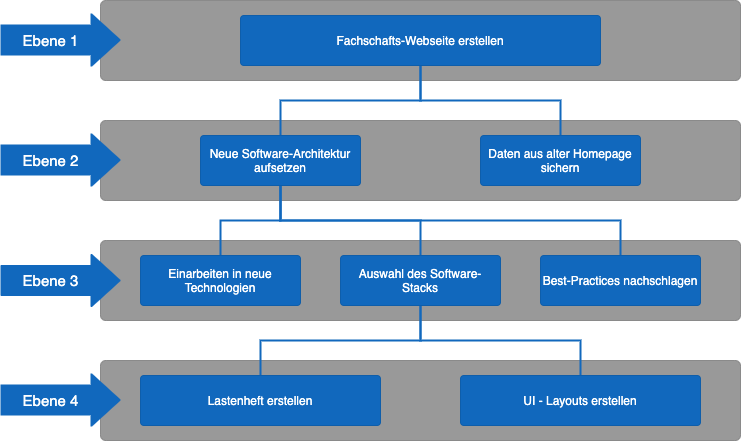
\includegraphics[width=\textwidth]{gfx/homepage}
	\caption{Zielhierarchie: \textit{Fachschafts-Webseite erstellen}}
\end{figure}

Da es sich hierbei um ein eher komplexes Thema handelt und evtl. die Zuarbeit von Kommilitonen benötigt ist der Zeitaufwand relativ hoch. Außerdem gibt es keinen festen Zeitpunkt zu dem das Projekt abgeschlossen sein muss, daher ist die Priorität eher niedrig.

\subsubsection{2. Ziel: Halbmarathon-Zeit verbessern}
Ein persönliches Ziel ist, die letztjährige Zeit beim “Maisel´s FunRun” Halbmarathon zu verbessern. Um dieses Ziel zu erreichen könnte man folgende Einteilung vornehmen:

\begin{figure}[htb]
	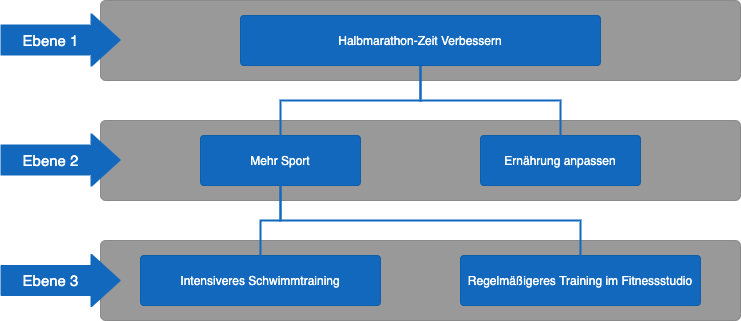
\includegraphics[width=\textwidth]{gfx/marathon}
	\caption{Zielhierarchie: \textit{Halbmarathon-Zeit verbessern}}
\end{figure}

Hier handelt es sich um einen langwierigen Prozess, für den gewisse Aufgaben regelmäßig wiederholt werden müssen. Diese können jedoch mit Hilfe von gutem Zeitmanagement in den Alltag integriert werden. Im Vergleich zum 1. Ziel existiert hier zwar ein fester Zeitpunkt, allerdings sind die Auswirkungen bei Erreichen eher gering. Aus diesem Grund ist die Priorität auch in diesem Fall eher niedrig.

\subsubsection{3. Ziel: Studium abschließen}
Dieses Ziel ist angelehnt an das Beispiel im Kurs, wurde allerdings deutlich konkretisiert. Um das Studium abzuschließen gilt es neben dem bestehen der beiden verbleibenden Module (Theoretische Informatik und diesem VHB Kurs) noch die Bachelorarbeit abzugeben. Da diese in Kooperation mit dem betreuenden Lehrstuhl und einem Unternehmen entsteht, existieren auch hier zusätzliche Abhängigkeiten:

\begin{figure}[htb]
	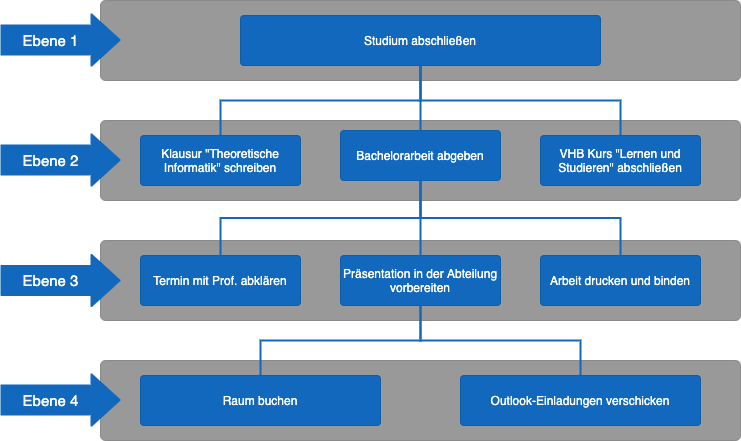
\includegraphics[width=\textwidth]{gfx/studium}
	\caption{Zielhierarchie: \textit{Studium abschließen}}
\end{figure}

Das Erreichen dieses Ziels hat sowohl deutliche Auswirkungen, als auch eine feste Deadline. In der hier aufgeführten Liste handelt es sich daher um das wichtigste und ist daher jenes Ziel mit der höchsten Priorität.

\subsubsection{4. Ziel: Buchreihe fertig lesen}
Zum herstellen einer vernünftigen Work-Life-Balance und um zu Vermeiden nur noch an Projekten für Arbeit und / oder Studium zu arbeiten wurde als persönliches Ziel festgehalten, die bereits begonnene Buchreihe “Der dunkle Turm” von Stephen King zu ende zu lesen.

\begin{figure}[htb]
	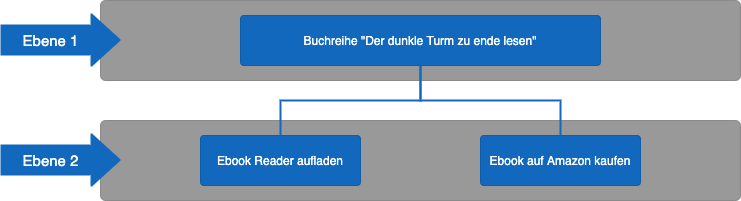
\includegraphics[width=\textwidth]{gfx/buchreihe}
	\caption{Zielhierarchie: \textit{Buchreihe fertig lesen}}
\end{figure}

Auch hier handelt es sich um ein Ziel mit keinem festen Zeitpunkt. Zudem ist hier sprichwörtlich eher “der Weg das Ziel”. Das heißt, die Auswirkungen beim tatsächlichen Erreichen sind sehr gering. Somit ist dieses Ziel, dasjenige welches die geringste Priorität in der Liste hat.

\subsubsection{5. Ziel: Schlafzimmer renovieren}
Um den eigenen Wohnkomfort zu erhöhen wurde das Ziel gefasst, im Schlafzimmer neuen Parkett-Boden zu verlegen und die Wände neu zu streichen.

\begin{figure}[htb]
	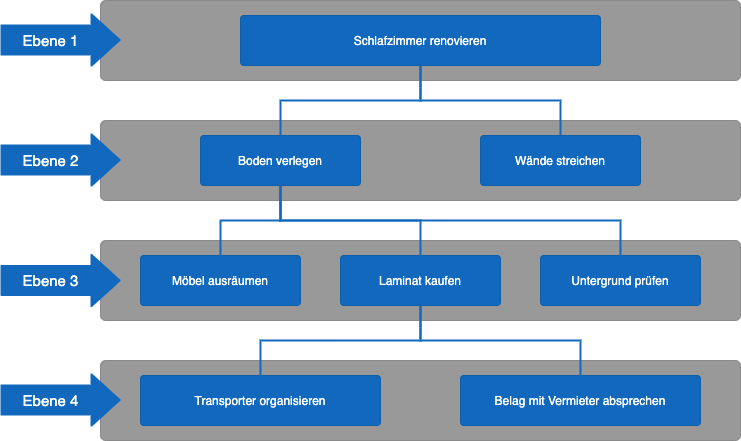
\includegraphics[width=\textwidth]{gfx/renovieren}
	\caption{Zielhierarchie: \textit{Schlafzimmer renovieren}}
\end{figure}

Dieses Ziel besitzt zwar ebenfalls keinen Zeitpunkt zu dem es zwangsläufig erreicht sein muss, jedoch hat es eine deutliche Auswirkung wenn die entsprechenden Aufgaben bzw. Arbeiten abgeschlossen wurden.Der Zeitaufwand hält sich außerdem verhältnismäßig in Grenzen, sodass dieses Ziel mit mittlerer Priorität bewertet wird.

% !TEX root = ../lust-1.tex
%
\chapter{Lernen und Aufmerksamkeit}
\label{sec:lernen-und-aufmerksamkeit}

\paragraph{Teil 3 der Hausarbeit}
Stellen Sie sich vor, dass ein Freund während der Prüfungsphase zu Ihnen kommt und Rat sucht, da er Probleme hat beim Lernen. Was würden Sie ihm raten und warum? Nehmen Sie hierbei Bezug auf die im Modul besprochenen endogenen Einflüsse und Umwelteinflüsse. \\[0.4em]

Zunächst ist einmal anzuraten, die Ursache der Probleme herauszufinden. Probleme beim Lernen können durch viele (auch unbewusste) Faktoren auftreten.

Ein Grund für Ineffektivität beim Lernen kann beispielsweise Schlafdeprivation sein. Nicht ohne Grund existiert im Arbeitszeitgesetz der Paragraph Nr. 5 nach dem Arbeitnehmer zwischen zwei Arbeitstagen mindestens 11h Ununterbrochene Ruhezeit bekommen müssen. Entsprechend sollte man auch zwischen Lerntagen / Lernphasen genügend Ruhezeit einhalten. Die Menge an benötigten Schlaf variiert von Mensch zu Mensch, sollte im Mittel jedoch zwischen 6 und 8 Stunden pro Nacht (für einen Erwachsenen) betragen.
Des weiteren ist zu beachten, dass Schlaf nicht “angespart” werden kann.

Ein weiterer Einflussfaktor können vorübergehende Erkrankungen sein. Dazu zählen auch physische Erkrankungen wie beispielsweise ein gebrochenes Bein. Auch in diesem Fall kann die Lerneffizienz stark beeinflusst sein. Entsprechend ist dem Erkrankten zu empfehlen sich selbst zunächst auszukurieren.

Die (übermäßige) Einnahme psychoaktiver Substanzen kann ebenfalls zu einbußen der Effektivität beim Lernen führen. Rauschmittel wie Alkohol, Koffein, illegale Suchtdrogen, aber auch gewisse Medikamente besitzen keine aktivierungsfördernde Wirkung, sondern gehen meistens mit einer massiven Dämpfung des Leistungsvermögens einher.

Sollten die genannten endogenen Einflüsse bereits berücksichtig werden können auch (unterbewusst) exogene Einflüsse das Lernen beeinflussen.

Der Wechsel des Lernplatzes könnte beispielsweise eine Steigerung der Effektivität mit sich bringen. Konkret könnte man versuchen statt zu Hause am Schreibtisch zu lernen in die Uni-Bibliothek zu gehen. Der Lernort besitzt viele Faktoren, die den Lernfortschritt beeinflussen (Temperatur, Beleuchtung, etc.). Daher. kann es unter Umständen auch schon helfen zu Hause vom Schreibtisch an den Esstisch zu wechseln (oder umgekehrt).

Eine weitere Möglichkeit ist, mit Hilfe von bestimmten Ritualen, sich mental auf das Lernen vorzubereiten. Dies kann dabei helfen die Umstellung von Freizeit zu Arbeitsphasen zu erleichtern.

% !TEX root = ../lust-1.tex
%
\chapter{Lernprinzipien}
\label{sec:lernprinzipien}

\paragraph{Teil 4 der Hausarbeit}
Überlegen Sie sich ein Lernbeispiel und beschreiben Sie, wie das Lernen in diesem Beispiel ablief. Nehmen Sie hierbei Bezug auf die im Modul besprochene Lernkurve und ihre Charakteristika. Stellen Sie diesem Beispiel eines gegenüber, bei dem Lernen durch Einsicht vorlag. Was waren Unterschiede und was vielleicht Gemeinsamkeiten? Was hat Ihnen mehr Spaß gemacht und warum? … \\[0.4em]

Ein Beispiel für einen Lernvorgang, welcher der Lernkurve nach Ebbinghaus folgt ist das Erlernen einer neuen Programmiersprache (unter der Voraussetzung, dass man bereits programmieren kann). Hier wurden zunächst essenzielle Teile gelernt. Diese umfassen beispielsweise:

\begin{itemize}
    \item Das erstellen von Variablen / Konstanten
    \item Die Definition von Funktionen / Methoden
    \item Das ausführbar machen (engl. compile) des geschriebenen Quellcodes
\end{itemize}

Somit wird sehr schnell ein großer Fortschritt im Lernprozess erzielt, da an dieser Stelle bereits einfache Funktionalität umgesetzt werden kann.

Im Anschluss wurde mehr über die Struktur und den Aufbau der Sprache gelernt. Besonders interessant waren hierbei die möglichen Programmierparadigmen (Objektorientierung, Funktionalität, Aspektorientierung, Prozeduralität, etc.). Dazu kommt das Lernen von Erweiterbarkeit und wie Bibliotheken (also Code anderer Entwickler) genutzt werden können, um komplexere Funktionalitäten umzusetzen, bzw. den eigenen Programmieraufwand zu reduzieren.
Hier fängt der Lernfortschritt an zu stagnieren.

Mit genügend Übung können zum Schluss komplette Anwendungen mit komplexer Funktionalität implementiert werden, wobei “nur” noch Maßnahmen zur Speicher- und Laufzeitoptimierung gelernt werden. Der Fortschritt ist also nur noch sehr gering.

Anders verläuft der Lernvorgang beim verstehen des Induktionsbeweises in der Mathematik.
Hier mussten zunächst etliche Beispielaufgaben betrachtet werden, um die formale Struktur des Beweises nachzuvollziehen bzw. zu verstehen. Die Reproduktion des Beweises ist danach allerdings unabhängig von der Problemstellung möglich.

Die beiden Beispiele unterscheiden sich darin, dass bei ersterem das Lernen schrittweise erfolgt ist, während bei letzterem das Gesamtkonzept verstanden werden musste. Ein weiterer Unterschied ist, dass durch das Lernen einer wieder neuen Programmiersprache die Syntax der alten schneller verdrängt wird, wohingegen der Induktionsbeweis trotz lernen anderer Beweistechniken reproduzierbar bleibt.

Als Gemeinsamkeit lässt sich festhalten, dass beide Lernbeispiele zunächst geübt werden mussten um sie zu verinnerlichen. Außerdem wurde das Lernen beider Beispiele durch Hilfsmittel wie Videos und Vorlesungsskripte unterstützt.

Grundsätzlich hat das lernen der Programmiersprache mehr Spaß gemacht, da hier schrittweise kleine Zwischenerfolge erzielt wurden. Außerdem motiviert die Tatsache immer noch eine Kleinigkeit dazu lernen zu können.

% !TEX root = ../lust-1.tex
%
\chapter{Lernstrategien}
\label{sec:lernstrategien}

\paragraph{Teil 5 der Hausarbeit}
Welche Erfahrungen haben Sie bereits bezüglich Erfahrung und Lernen gemacht? Gab es hier positive und negative Beispiele, wie Erfahrung Ihr Lernen beeinflusst hat? Welche Lernstrategien nutzen Sie am häufigsten und wie effektiv sind diese Strategien für Sie? Nehmen Sie hierbei Bezug auf die im Modul bearbeiteten Inhalte. \\[0.4em]

Zu den bevorzugten Lernstrategien zählt zunächst das nutzen des Vorwissens um evt. komplexere Sachverhalte eigenständig herleiten zu können. Mathematische Formeln müssen dadurch also nicht (oder nur zum Teil) auswendig gelernt werden. Zusätzlich ermöglicht das bereits vorhandene Wissen die Bildung von Eselsbrücken, um sich andere / fremde Inhalte einfacher einprägen zu können.

Am häufigsten werden jedoch Notizen zum Lernen genutzt. Diese beinhalten Stichpunktartig die wichtigsten Informationen, komprimiert auf möglichst wenig Zeichen. Ein wichtiger Faktor ist, dass diese Zusammenfassungen handschriftlich und nicht maschinell erstellt werden, da dies den Lernprozess bereits vorantreibt. Unterstützt werden können die Notizen durch entsprechende Grafische Anordnungen und Diagramme.

% !TEX root = ../lust-1.tex
%
\chapter{Problemlösen}
\label{sec:problemloesen}

\paragraph{Teil 6 der Hausarbeit}
Ein Freund plant einen Urlaub und hat aber nur ein bestimmtes Reisebudget. Er möchte gerne nach Südamerika fliegen und dort für 3 Wochen verschiedene Orte besuchen. Der Flug nach Südamerika ist bereits sehr teuer und jetzt weiß er nicht, wie er das Problem des begrenzten Budgets am besten lösen kann, um das meiste aus dem Urlaub holen zu können. Er sucht nach Rat bei Ihnen. Analysieren Sie den Problemlöseprozess (Problemlöseschritte) anhand dieses Beispiels. Was würden Sie ihm raten? \\[0.4em]

Der Problemlöseprozess besteht aus den 5 Schritten:

\begin{enumerate}
    \item Ausgangszustand formulieren
    \item Zielzustand definieren
    \item Mögliche Lösungswege erörtern
    \item Entscheidung für einen Weg treffen
    \item Durchführen und Evaluieren der Entscheidung
\end{enumerate}

Der Ausgangszustand beinhaltet die Planung eines Urlaubs, für welchen jedoch nur ein begrenztes Budget zur Verfügung steht.

Zielzustand ist möglichst viel Gegenwert für das bezahlte Geld zu bekommen.

Mögliche Lösungswege wären beispielsweise:

\begin{itemize}
    \item Andere Transportmittel nutzen
    \item Die Reisezeit verkürzen
    \item Das Reiseziel zu ändern
    \item Auf der Reise Geld verdienen (Work \& Travel, Remote-Arbeiten, etc.)
    \item Länger sparen / Reise verschieben
    \item Geld leihen
\end{itemize}

Als Ratschlag würde ich geben entweder die Reisezeit zu verkürzen, d.h. an das entsprechende Budget anzupassen, oder das Reiseziel zu ändern. Bei letzterem würde unter Umständen auch beispielsweise die Möglichkeit bestehen andere Transportmittel zu nutzen.
Sollte keiner der beiden Lösungswege eine Option sein ist die sinnvollste Alternative die Reise zu einem späteren Zeitpunkt und mit mehr (finanziellen) Ressourcen anzutreten.

% !TEX root = ../lust-1.tex
%
\chapter{Kommunikation}
\label{sec:kommunikation}

\paragraph{Teil 7 der Hausarbeit}
Stellen Sie sich vor, Sie sind in sozialen Situationen sehr schüchtern und würden gerne die Kommunikation in sozialen Situationen gestalten. Welche Techniken könnten Sie hier anwenden? Beschreiben Sie diese konkret an Beispielen. Nehmen Sie Bezug zum im Modul behandelten Stoff. \\[0.4em]

Die Zielorientierung ist ungemein wichtig in der Kommunikationsgestaltung. Erreicht werden kann dies durch konkretes ausformulieren des Ziels und anschließendem Mitteilen an den Kommunikationspartner. Ein konkretes Beispiel könnte sein, dass man mit einem Kommilitonen ein Gespräch über Probleme mit dem eigenen Partner führen möchte.
In diesem Fall ist es beispielsweise zielführender das Gespräch zu beginnen mit “Ich habe ein Problem und hätte gerne einen Ratschlag von dir” als sich einfach aus heiterem Himmel über den Partner zu beschweren. Der Kommunikationspartner weiß bei ersterem schon vor dem eigentlichen Inhalt der Kommunikation was von ihm erwartet wird.

Als weiterer wichtiger Punkt gilt die Reziprozität, also das Gleichgewicht der Redeanteile. Dies kann unter Anderem durch Nachfragen erzielt werden.
Vorstellen könnte man sich beispielsweise ein Gruppengespräch über ein Thema, welches für einen selbst noch relativ neu ist. Bevor man in diesem Fall mit Halbwissen in das Gespräch versucht einzubringen ist es sinnvoller bei Unklarheiten nachzufragen.

Ein dritter Faktor sind die sogenannten “Ich”-Formulierungen. Diese sollen die eigene Meinung in einem Gespräch widerspiegeln. Ein Beispiel hierfür wäre eine Gruppenarbeit bei der man mit der Leistung des Kommilitonen unzufrieden ist und diesen entsprechend darauf hinweisen möchte. Anstatt die Konversation zu beginnen mit “Das hättest du detaillierter formulieren können” könnte man sich besser wie folgt ausdrücken “Ich hätte diesen Teil etwas detaillierter formuliert”.


\cleardoublepage
% --------------------------
% Back matter
% --------------------------
%
{%
\setstretch{1.1}
\renewcommand{\bibfont}{\normalfont\small}
\setlength{\biblabelsep}{0pt}
\setlength{\bibitemsep}{0.5\baselineskip plus 0.5\baselineskip}
\printbibliography[nottype=online]
\newrefcontext[labelprefix={@}]
\printbibliography[heading=subbibliography,title={Webpages},type=online]
}

% \listoffigures
% \cleardoublepage

% \listoftables
% \cleardoublepage

% \lstlistoflistings
% \cleardoublepage

%\appendix\cleardoublepage
%% !TEX root = ../lust-2.tex
%
\chapter{Anhang}
\label{sec:appendix}

\section{Exzerpt zu Lernen mit Texten}
\label{sec:appendix:sec1}

\includegraphics[width=\textwidth,page=1]{gfx/endliche-automaten}
\clearpage
\includegraphics[width=\textwidth,page=3]{gfx/endliche-automaten}
\clearpage
\includegraphics[width=\textwidth,page=4]{gfx/endliche-automaten}
\clearpage
\includegraphics[width=\textwidth,page=5]{gfx/endliche-automaten}
\clearpage
\includegraphics[width=\textwidth,page=6]{gfx/endliche-automaten}
\clearpage
\includegraphics[width=\textwidth,page=7]{gfx/endliche-automaten}
\clearpage
\includegraphics[width=\textwidth,page=8]{gfx/endliche-automaten}
\clearpage
\includegraphics[width=\textwidth,page=9]{gfx/endliche-automaten}
\clearpage
\includegraphics[width=\textwidth,page=10]{gfx/endliche-automaten}
\clearpage
\includegraphics[width=\textwidth,page=11]{gfx/endliche-automaten}       % INCLUDE: appendix

\clearpage

%\newpage
%\mbox{}

% **************************************************
% End of Document CONTENT
% **************************************************
\end{document}
